

\section{Введение}
\subsection{Цель работы}
Целью данной лабораторной работы является исследование и анализ характеристик чувствительности осциллографа, а также изучение фигур Лиссажу для разных отношений частот. В процессе работы будет выполнен расчет максимальной чувствительности, коэффициента усиления, а также проведены эксперименты для определения отклонений и их влияния на точность измерений.

\subsection{Решаемые задачи}
\begin{enumerate}
  \item Исследовать чувствительность пластин вертикального и горизонтального отклонений осциллографической трубки. 
  \item Наблюдать с помощью осциллографа синусоидальное напряжение, полученное с выхода генератора. 
  \item Получить фигуры Лиссажу и определить частоту исследуемого напряжения по фигурам Лиссажу.
\end{enumerate}

\section{Основная часть}

\subsection{Теоретическая часть}

\paragraph{Измерения}
Чувствительность горизонтальных и вертикальных пластин измеряется по формуле:
\begin{equation}
S = \frac{L}{2 \sqrt{2} \cdot U_{\text{eff}}}
\end{equation}
где \begin{itemize}
    \item \( S \) — чувствительность (мм/В),
    \item \( L \) — длина одного деления экрана осциллографа,
    \item \( U_{\text{eff}} \) — эффективное напряжение.
\end{itemize}


\subsection{Эксперимент}
Для получения термоэлектронной эмиссии катод трубки нагревают, подавая на нагреватель катода переменное напряжение. Вылетевшие из катода электроны ускоряются электрическим полем и движутся по направлению к аноду. По пути они пролетают через фокусирующей электрод, который собирает вылетевшие электроны в пучок, образуя электронный луч, который проходит между отклоняющими пластинами двух взаимно перпендикулярных плоских конденсаторов. Если в конденсаторах создать электрическое поле, то первый конденсатор С1 может отклонять луч в одном направлении, а второй конденсатор С2 – в перпендикулярном. Пройдя отклоняющие пластины конденсаторов, электронный луч попадает в широкую часть трубки. Экран электронно-лучевой трубки покрывается веществом, которое светится под действием электронного пучка. В результате на экране видно светящееся пятно F. При правильно подобранных напряжениях на катоде, аноде и фокусирующем электроде это пятно имеет размеры порядка 1 мм в диаметре.
\begin{figure}[ht!]
\centering
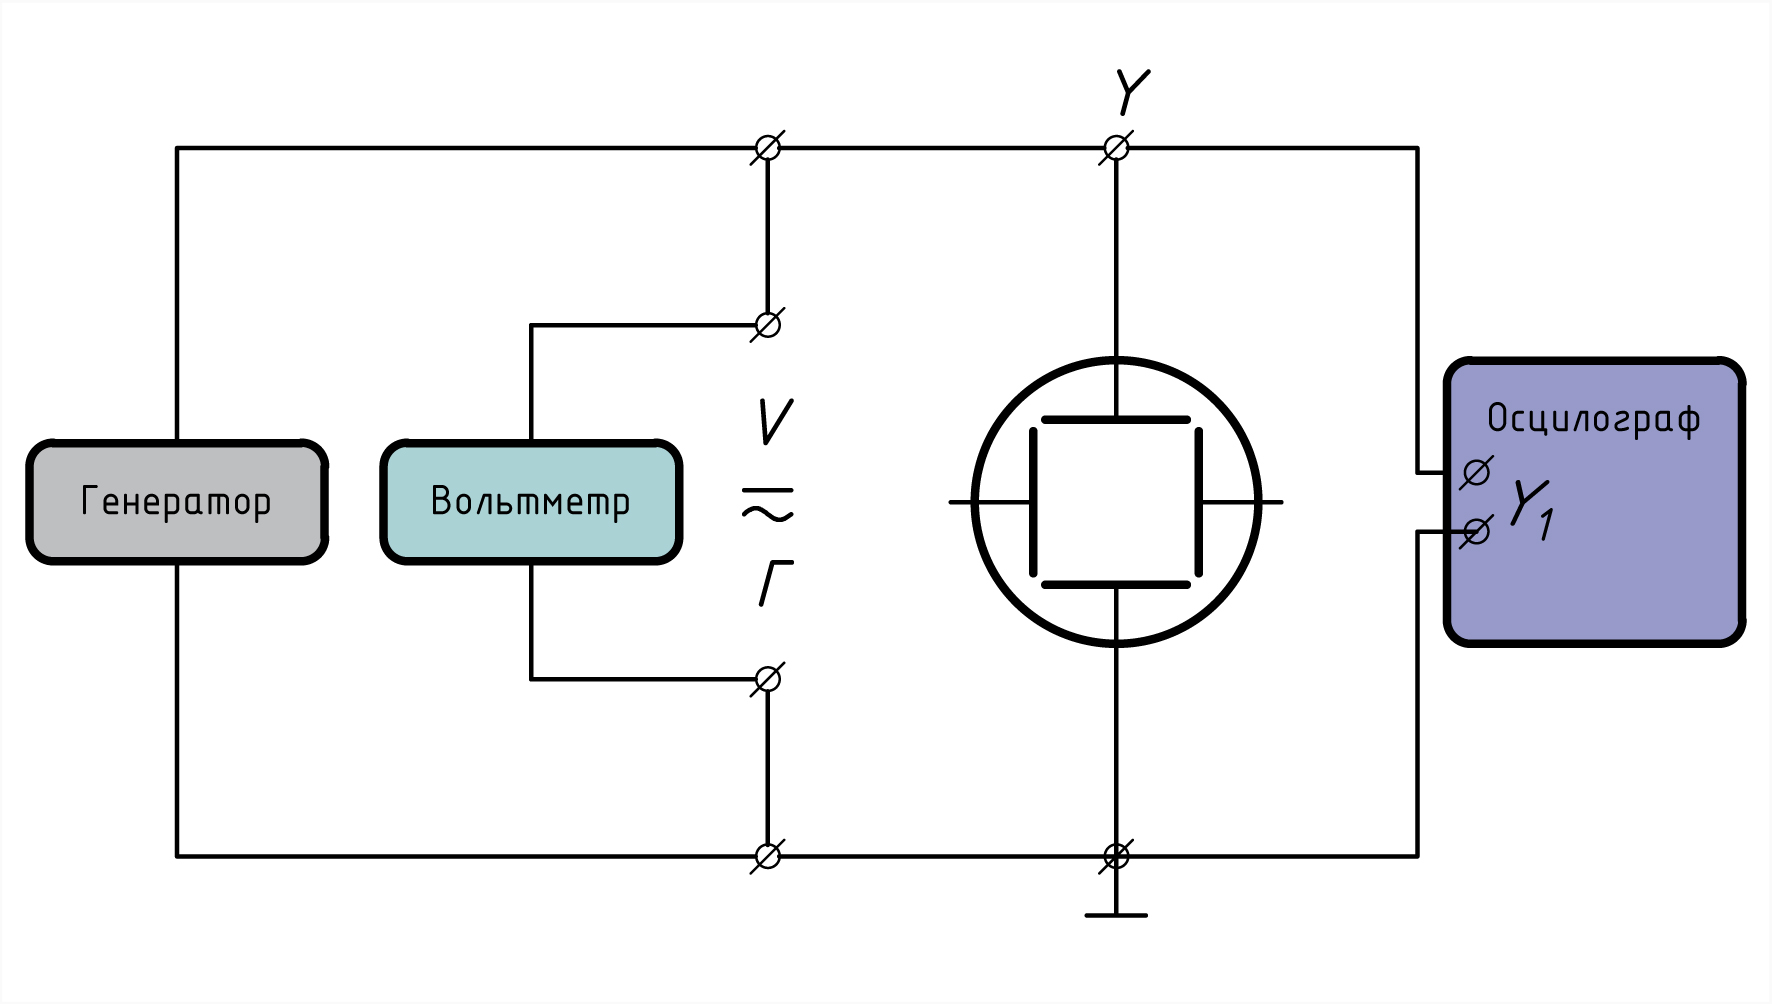
\includegraphics[width=0.6\textwidth]{1_Осцилограф-Лист1.jpg}
\caption{Схема установки}
\label{fig:sketch}
\end{figure}

\begin{figure}[ht!]
\centering
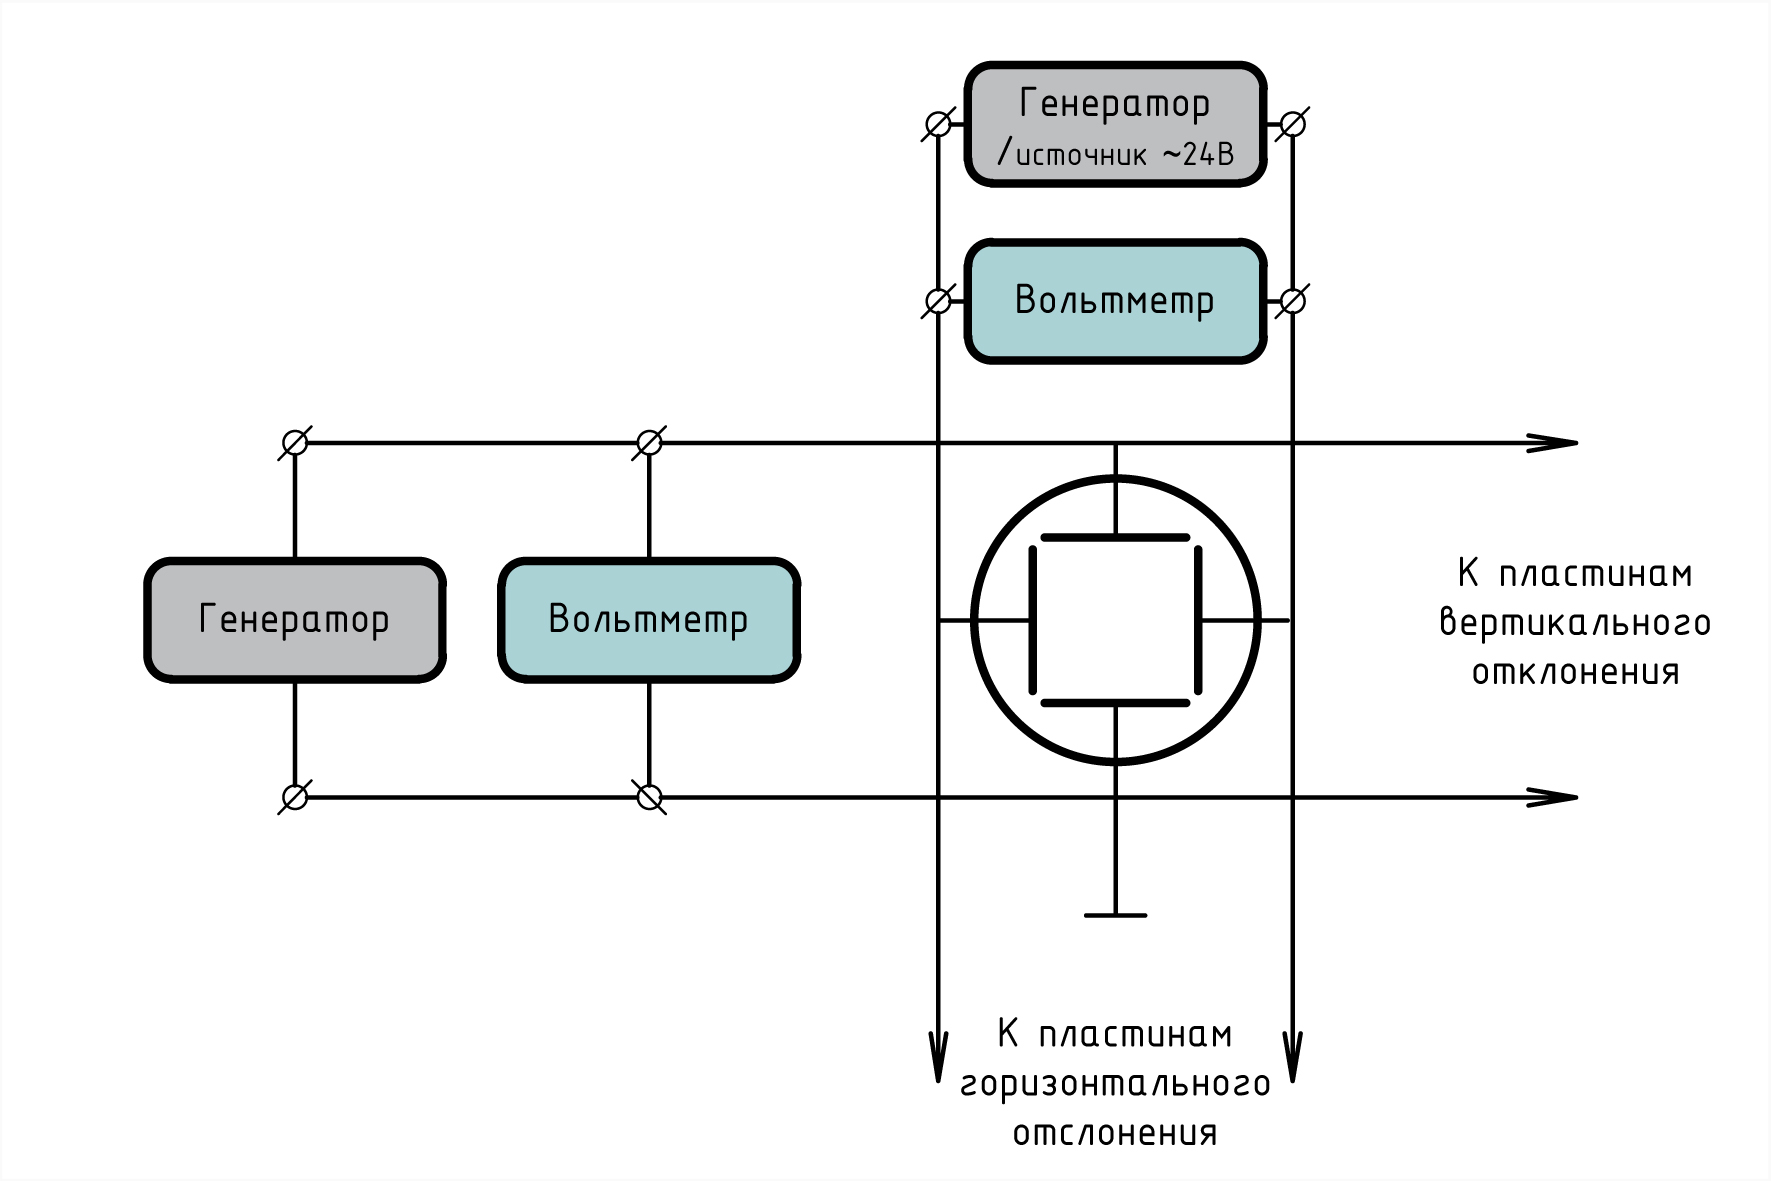
\includegraphics[width=0.6\textwidth]{2_Осцилограф-Лист1.jpg}
\caption{Схема установки}
\label{fig:sketch}
\end{figure}

\begin{figure}[ht!]
\centering
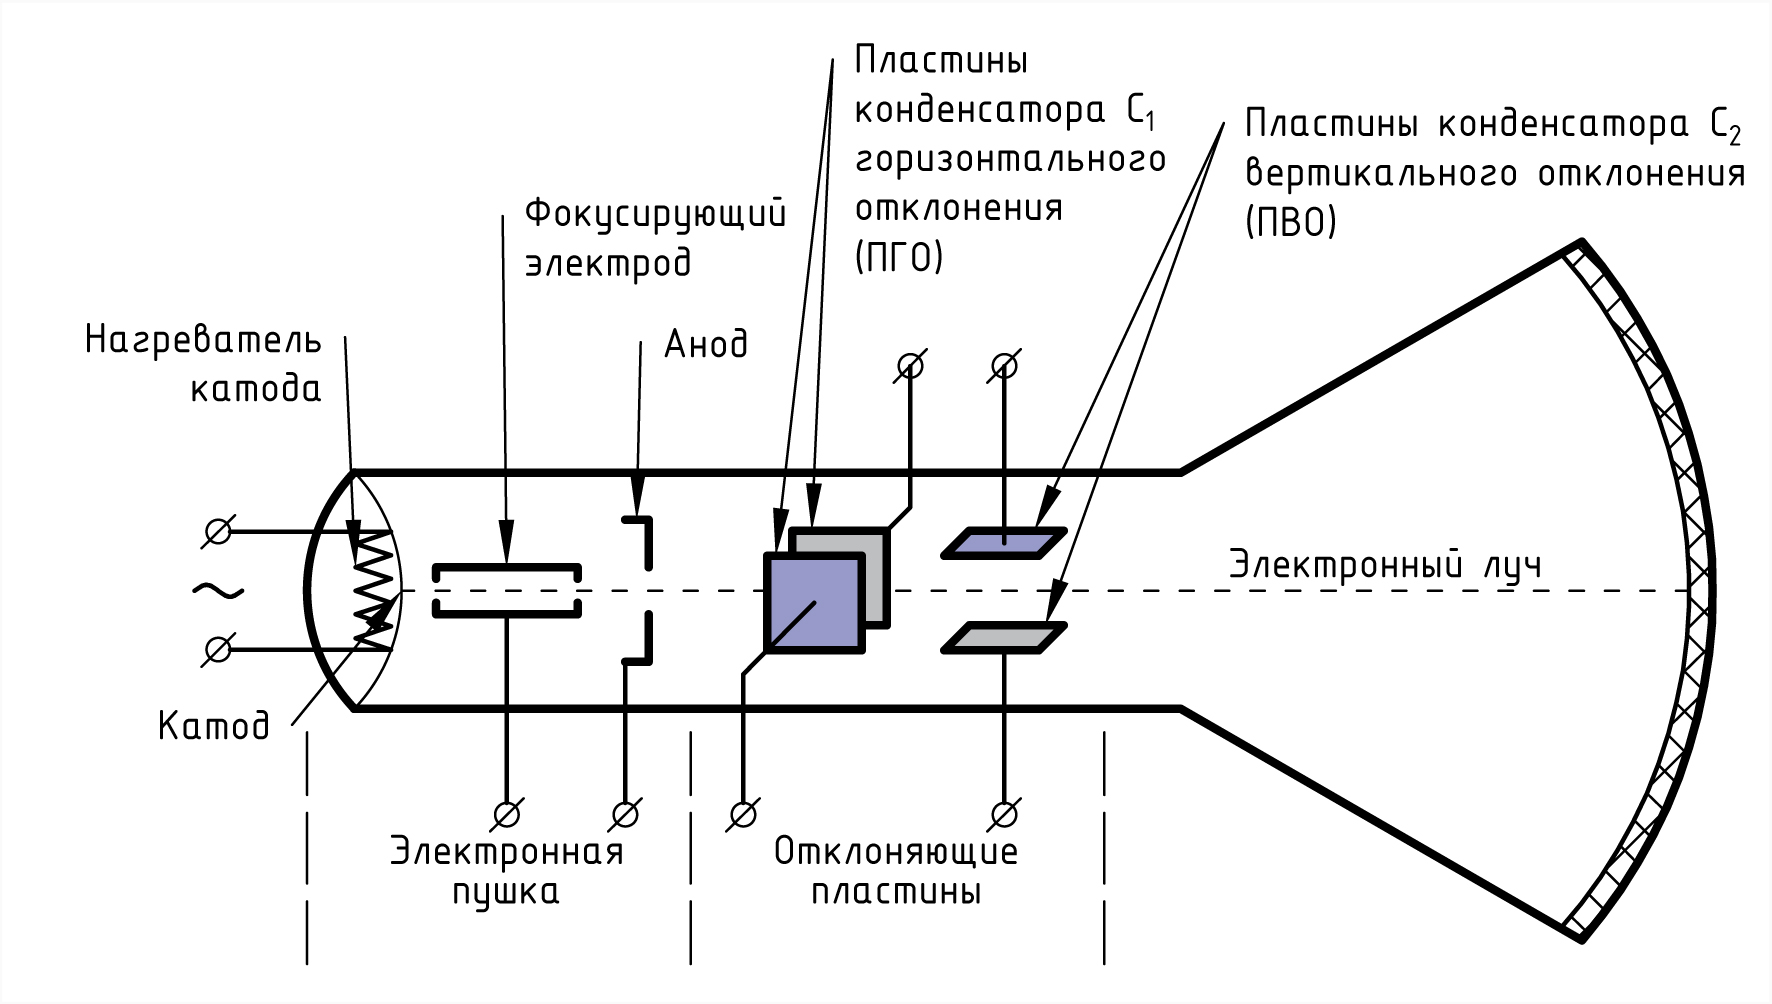
\includegraphics[width=0.8\textwidth]{3_Осцилограф-Лист1.jpg}
\caption{Схема установки}
\label{fig:sketch}
\end{figure}

\begin{figure}[H]
\centering
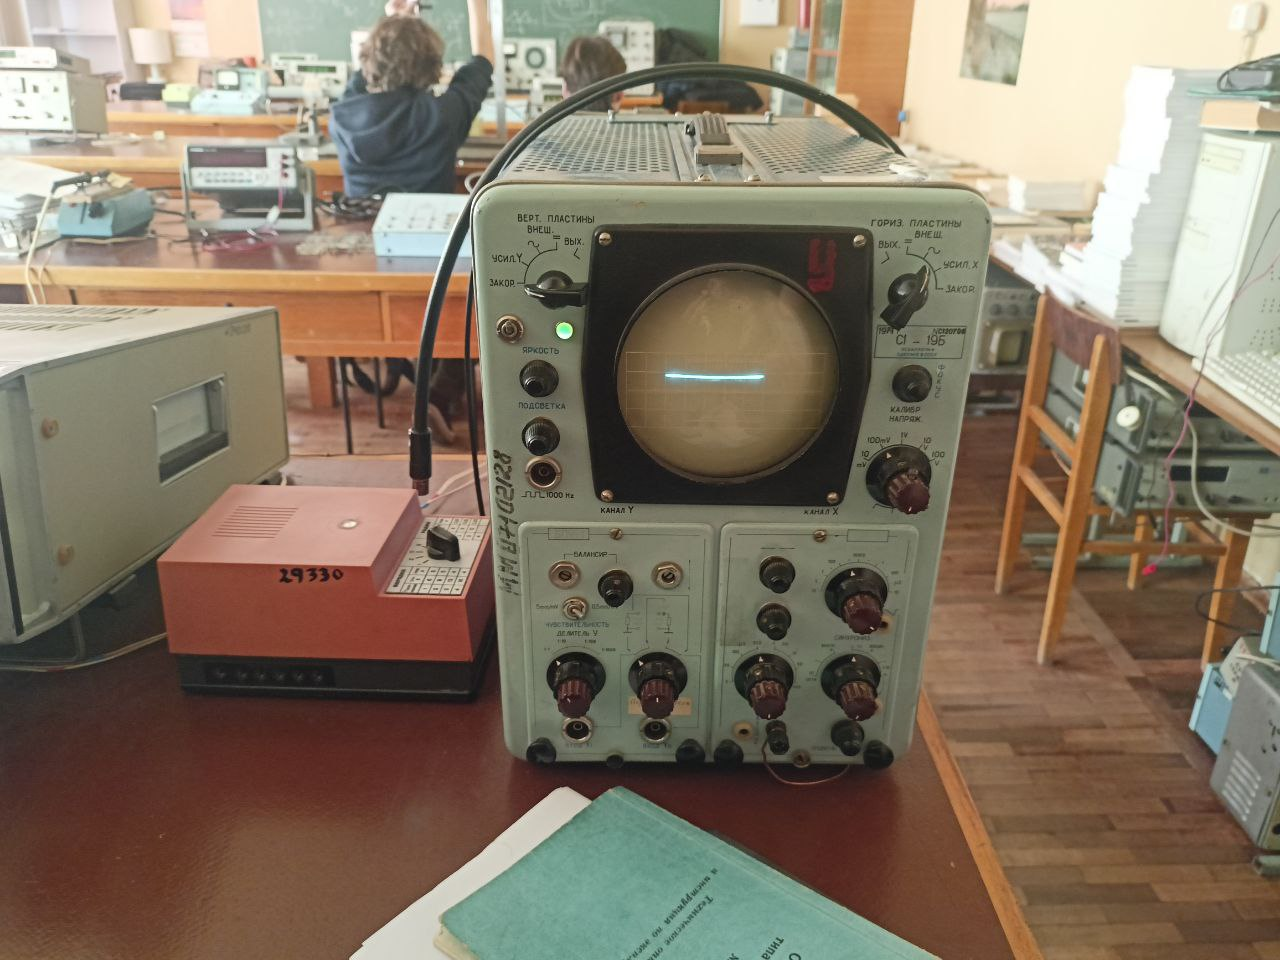
\includegraphics[width=0.6\textwidth]{1.jpg}
\caption{Фотография установки - осциллограф}
\label{fig:device}
\end{figure}

\begin{figure}[H]
\centering
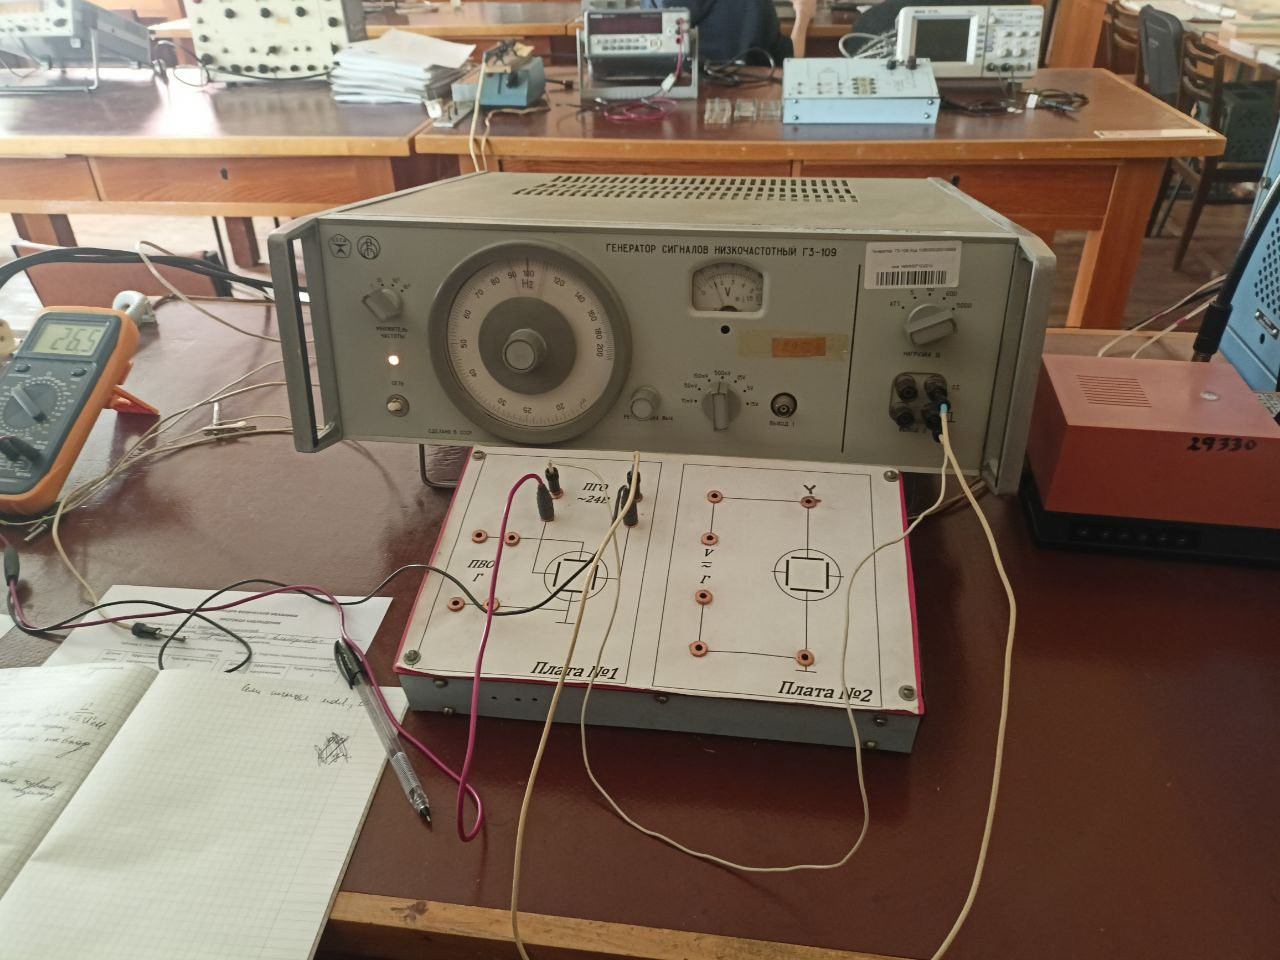
\includegraphics[width=0.6\textwidth]{2.jpg}
\caption{Фотография установки - генератор сигналов}
\label{fig:device}
\end{figure}


\subsection{Обработка данных и обсуждение результатов}

\subsubsection{Исходный код}
Для написания программы, вычисляющей все требуемые данные, используется язык C++; среда разработки - Visual Studio.

Программа на C++ выполняет следующие задачи:
\begin{enumerate}
    \item Читает данные из трех файлов: \texttt{Ueff\_vertical.txt}, \texttt{Ueff\_horizontal.txt}, \texttt{Ueff\_max.txt}, содержащих значения напряжений \( U_{eff} \).
    \item Рассчитывает чувствительность \( S \) по формуле:
    \[
    S = \frac{L}{2 \cdot \sqrt{2} \cdot U_{eff}}
    \]
    где \( L \) — длина, а \( U_{eff} \) — значение напряжения для каждой точки.
    \item Проверяет соответствие размеров массивов данных. В случае несоответствия выбрасывает исключение.
    \item Выводит результаты вычислений в консоль для вертикальных и горизонтальных данных и записывает результаты для данных из \texttt{Ueff\_max.txt} в файл \texttt{output\_max.txt}.
    \item Обрабатывает ошибки, такие как невозможность открыть файл или несоответствие размеров данных.
    \item Устанавливает кодировку консоли в UTF-8 для корректного отображения символов.
\end{enumerate}

\begin{lstlisting}[label=listing1, caption=Функция считывания данных из файла]
std::vector<double> readData(const std::string& filename) {
    std::ifstream file(filename);
    if (!file.is_open()) {
        throw std::runtime_error("Не удалось открыть файл " + filename);
    }

    std::vector<double> data;
    double value;
    while (file >> value) {
        data.push_back(value);
    }

    return data;
}

\end{lstlisting}

\begin{lstlisting}[label=listing2, caption=Функция расчета чувствительности]
std::vector<double> calculateSensitivity(const std::vector<double>& L, const std::vector<double>& Ueff) {
    std::vector<double> sensitivity;

    for (size_t i = 0; i < L.size(); ++i) {
        double S = L[i] / (2 * std::sqrt(2) * Ueff[i]);
        sensitivity.push_back(S);
    }

    return sensitivity;
}
\end{lstlisting}

\begin{lstlisting}[label=listing2, caption=Функция для вычисления среднего значения]
double mean(const vector<double>& data) {
    double sum = 0.0;
    for (double value : data) {
        sum += value;
    }
    return sum / data.size();

// Функция для вычисления стандартного отклонения (деление на n(n-1))
double standard_deviation(const vector<double>& data) {
    double avg = mean(data);
    double sum_squared_diff = 0.0;

    // Суммируем квадраты отклонений
    for (double value : data) {
        sum_squared_diff += pow(value - avg, 2);
    }

    // Стандартное отклонение (деление на n(n-1))
    return sqrt(sum_squared_diff / (data.size() * (data.size() - 1)));
}
\end{lstlisting}

\subsubsection{Таблицы}

\begin{table}[h!]
\centering
\resizebox{\textwidth}{!}{%
\begin{tabular}{|c|c|c|}
\hline
\textbf{Длина линии на экране, \( L \) (мм)} & \textbf{Эффективное напряжение, \( U_{\text{eff}} \) (В)} & \textbf{Чувствительность, \( S \) (мм/В)} \\
\hline
10 & 4,5 & 0.785674 \\
20 & 10,9 & 0,648722 \\
30 & 17,5 & 0,606092 \\
40 & 23,5 & 0,601793 \\
50 & 31,6 & 0,55942 \\
\hline
\end{tabular}
}
\caption{Опытные данные и чувствительность пластин вертикального отклонения (ПВО)}
\end{table}

\begin{table}[h!]
\centering
\resizebox{\textwidth}{!}{%
\begin{tabular}{|c|c|c|}
\hline
\textbf{Длина линии на экране, \( L \) (мм)} & \textbf{Эффективное напряжение, \( U_{\text{eff}} \) (В)} & \textbf{Чувствительность, \( S \) (мм/В)} \\
\hline
10 & 3 & 1.17851 \\
20 & 8,5 & 0.83189 \\
30 & 13,7 & 0.774205 \\
40 & 20,2 & 0.700106 \\
50 & 26,5 & 0,667082 \\
\hline
\end{tabular}
}
\caption{Опытные данные и чувствительность пластин горизонтального отклонения (ПГО)}
\end{table}

\begin{table}[h!]
\centering
\resizebox{\textwidth}{!}{%
\begin{tabular}{|c|c|c|}
\hline
\textbf{Длина линии на экране, \( L \) (мм)} & \textbf{Эффективное напряжение, \( U_{\text{eff}} \) (В)} & \textbf{Чувствительность, \( S \) (мм/В)} \\
\hline
10 & 0,073 & 48.432 \\
20 & 0,12 & 58.9256 \\
30 & 0,196 & 54.1153 \\
40 & 0,351 & 40.291 \\
\hline
\end{tabular}
}
\caption{Максимальная чувствительность осциллографа}
\end{table}

\begin{table}[h!]
\centering
\resizebox{\textwidth}{!}{%
\begin{tabular}{|c|c|c|c|c|}
\hline
\textbf{Вид фигуры Лиссажу} & o & 8 & ooo & oo \\
\hline
\textbf{Отношение частот} \( f_x/f_y \) & 1:1 & 2:1 & 1:3 & 1:2 \\
\hline
\textbf{Частота по лимбу генератора} \( f_y \), Гц & 50 & 25 & 150 & 100 \\
\hline
\textbf{Исследуемая частота} \( f_x \), Гц & 50 & 50 & 50 & 50 \\
\hline
\end{tabular}
}
\caption{Таблица исследования фигур Лиссажу}
\end{table}


\subsubsection{Графики}

\begin{figure}[ht!]
\centering
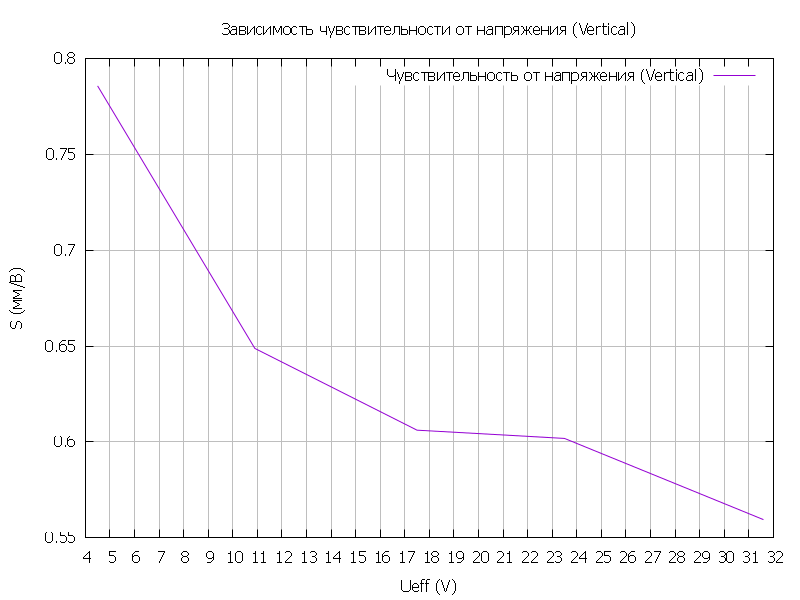
\includegraphics[width=0.8\textwidth]{SensVertical_graph.png}
\caption{Зависимость чувствительности пластин вертикального отклонения от напряжения}
\label{fig:plot}
\end{figure}

\begin{figure}[ht!]
\centering
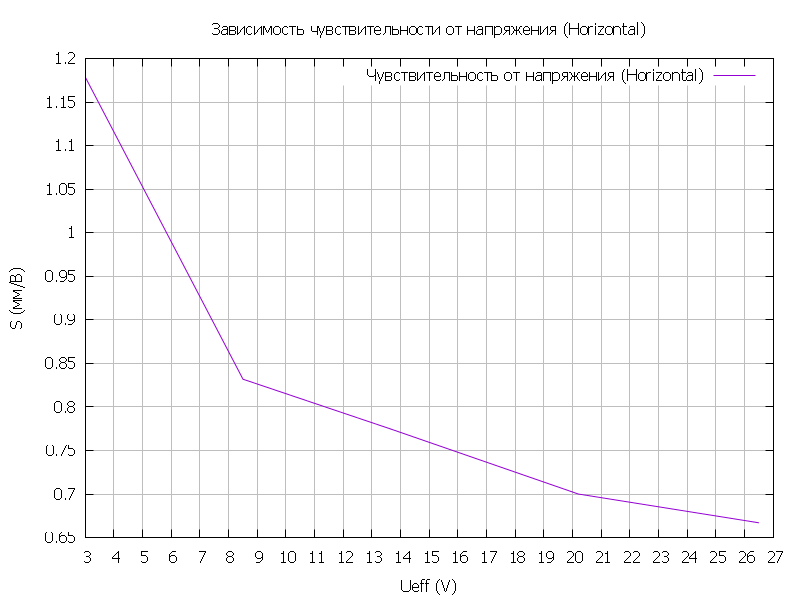
\includegraphics[width=0.8\textwidth]{SensHorizontal_graph.png}
\caption{Зависимость чувствительности пластин горизонтального отклонения от напряжения}
\label{fig:plot}
\end{figure}

Из графиков ПВО и ПГО видим, что ПВО в диапазоне 10,9 – 31,6, ПГО в диапазоне 8,5-26,5 находятся в зоне постоянной чувствительности. Вычислим значения как средние арифметические трех соответствующих измерений, и погрешность как стандартную погрешность этих измерений.
\[
S_y = 0.64034\, \text{мм/В}
\]
\[
S_x = 0.830359 \, \text{мм/В}
\]
\[
\Delta S = \sqrt{\frac{\sum_{i=1}^{n} (S_i - \overline{S})^2}{n(n-1)}}
\]

Таким образом:
\[
\Delta S_y = 0.0389866 \, \text{мм/В}, \quad \Delta S_x = 0.0916488 \, \text{мм/В}
\]

Максимальный коэффициент усиления:

\[
K_{\text{max}} = \frac{S}{S_y} = 92.022
\]


\section{Вывод}
Были исследованы чувствительности пластин вертикального и горизонтального отклонений осциллографической трубки. При синусоидальном напряжении были получены различные неподвижные фигуры Лиссажу, вычислено среднее напряжение, равное 50 ± 0,5 Гц.

% Список литературы
% Для отчёта он не обязателен
\begin{thebibliography}{9}

%ссылка на репозиторий с исходныим кодом отчета и всех расчетных программ обязательна 
\bibitem{repo}
\url{}  

\end{thebibliography}
\clearpage
\appendix